\documentclass{article}
\usepackage[latin1]{inputenc}
\usepackage{a4wide}
\usepackage{epsfig}
\usepackage{amssymb}
\usepackage{amsmath}
\usepackage{fancyvrb}
\usepackage{alltt}
\usepackage{fleqn}
\usepackage{epic}
\usepackage{color} 
\usepackage{theorem}
\usepackage{hyperref}
\usepackage[all]{hypcap}
\hypersetup{
        colorlinks = true, % comment this to make xdvi work
        linkcolor  = blue,
        citecolor  = red,
        filecolor  = [rgb]{0.1, 0.1, 1.0},
        urlcolor   = [rgb]{0.1, 0.1, 1.0},
        pdfborder  = {0 0 0} 
}

\usepackage{fancyhdr}
\usepackage{lastpage} 

\pagestyle{fancy}

\fancyfoot[C]{--- \thepage/\pageref{LastPage}\ ---}

\fancypagestyle{plain}{%
\fancyhf{}
\fancyfoot[C]{--- \thepage/\pageref{LastPage}\ ---}
\renewcommand{\headrulewidth}{0pt}
}

%\renewcommand{\chaptermark}[1]{\markboth{\chaptername \ \thechapter.\ #1}{}}
\renewcommand{\sectionmark}[1]{\markright{\thesection. \ #1}{}}
\fancyhead[R]{\leftmark}
\fancyhead[L]{\rightmark}

\definecolor{amethyst}{rgb}{0.2, 0.4, 0.6}
\definecolor{orange}{rgb}{1, 0.9, 0.0}

{\theorembodyfont{\sf}
\newtheorem{Definition}{Definition}
\newtheorem{Axiom}[Definition]{Axiom}
\newtheorem{Notation}[Definition]{Notation}
\newtheorem{Lemma}[Definition]{Lemma}
\newtheorem{Theorem}[Definition]{Theorem}
}

\newcommand{\proof}{\vspace*{0.2cm}

\noindent
\textbf{Proof}: }
 
\newcommand{\qed}{\hspace*{\fill} $\Box$
\vspace*{0.2cm}

}

\newcommand{\eod}{\hspace*{\fill} $\diamond$
\vspace*{0.2cm}

}

\newcommand{\eox}{\hspace*{\fill} $\diamond$
\vspace*{0.2cm}

}

\newcommand{\solution}{\vspace*{0.2cm}

\noindent
\textbf{Solution}: }

\newcounter{exercise}
\newcommand{\exercise}{\vspace*{0.2cm}
\stepcounter{exercise}

\noindent
\textbf{Exercise \arabic{exercise}}: }

\newcommand{\example}{\vspace*{0.2cm}

\noindent
\textbf{Example}: \ }

\newcommand{\examples}{\vspace*{0.2cm}

\noindent
\textbf{Examples}: \ }
 
\newcommand{\remark}{\vspace*{0.2cm}
\noindent
\textbf{Remark}: }

\newcommand{\lb}{\hspace*{\fill} \linebreak}

\newcommand{\bruch}[2]{\displaystyle\frac{\;\displaystyle#1\;}{\;\displaystyle#2\;}}
\newcommand{\bruchs}[2]{\textstyle\frac{\;\textstyle#1\;}{\;\textstyle#2\;}}
\newcommand{\bint}{\displaystyle\int}
\newcommand{\dint}[2]{\displaystyle\int_{#1}^{#2}\hspace{-0.2cm}}
\newcommand{\Oh}{\mathcal{O}}
\newcommand{\df}{\displaystyle\frac{d\;}{dx}}
\newcommand{\ds}{\displaystyle}
\newcommand{\norm}[1]{\big\|#1\bigr\|_{\infty}}

\def\pair(#1,#2){\langle #1, #2 \rangle}

\newlength{\mylength}
\setlength{\mathindent}{1.3cm}

\title{SymPy \& SciPy \\[0.3cm]
      --- An Appetizer --- } 
\author{Karl Stroetmann} 
\date{\today}
 
\begin{document}
\maketitle
\tableofcontents

\section{Preliminary Remarks}
This tutorial demonstrates some of the most important features of \href{http://sympy.org/en/index.html}{\textsl{SymPy}}
and \href{http://www.scipy.org}{\textsl{SciPy}}.  \textsl{SymPy} and \textsl{SciPy} are modules that extend the
programming language \href{http://www.python.org}{\textsl{Python}}.  
\begin{enumerate}
\item \textsl{SymPy} supports symbolic mathematics, i.e.~it can be used to solve equations symbolically, or for symbolic
      integration. 
\item \textsl{SciPy} implements a large number of numerical routines.
\end{enumerate}
Both of the packages can be used without prior knowledge of the programming language \textsl{Python}.
In this short paper we do not have the time to describe either \textsl{SymPy} or \textsl{SciPy} exhaustively.  Rather,
the idea is to arise the curiosity of the reader by describing some of the most interesting features.

\subsection{Installation}
This tutorial assumes that both \textsl{Python} and
\textsl{SymPy} have been installed.  \textsl{Python} can be installed  by following the instructions given on  
\\[0.2cm]
\hspace*{1.3cm}
\href{https://www.python.org/download/}{\texttt{https://www.python.org/download/}}.
\\[0.2cm]
The module \textsl{SymPy} can be found at
\\[0.2cm]
\hspace*{1.3cm}
\href{http://docs.sympy.org/latest/install.html}{\texttt{http://docs.sympy.org/latest/install.html}}
\\[0.2cm]
and the module \textsl{SciPy} is available at
\\[0.2cm]
\hspace*{1.3cm}
\href{http://www.scipy.org/install.html}{\texttt{http://www.scipy.org/install.html}}
\\[0.2cm]
Alternatively, \textsl{Python}, \textsl{SciPy}, and \textsl{SymPy} can be installed via 
\href{https://store.continuum.io/cshop/anaconda/}{\emph{Anaconda}}.  This is a lot simpler than installing
\textsl{Python}, \textsl{SciPy}, and \textsl{SymPy} separately.  The reason is that many systems (notably \textsl{Linux}
and \textsl{Mac OS X})  already have \textsl{Python} preinstalled, since a lot of other packages depend
on it.  Fiddling around with the preinstalled version of \textsl{Python} can compromise the
stability of the system.

\section{Introduction to \textsl{SymPy}}
\textsl{SymPy} is the module that supports symbolic computation.  In particular, \textsl{SymPy} is able to
\begin{enumerate}
\item perform symbolic differentiation and integration,
\item compute limits,
\item compute closed expressions for both finite sums and infinite  series,
\item solve ordinary equations, recurrence equations, and differential equations.
\end{enumerate}
We will demonstrate all these features in the following subsections.

To start \textsl{SymPy}, start a python interpreter by typing either the command \texttt{python} or \texttt{ipython} 
on the command line and issue the following command:
\\[0.2cm]
\hspace*{1.3cm}
\texttt{import sympy as sym}
\\[0.2cm]
Now all functions $f()$ defined in the package \texttt{sympy} can be accessed as
\\[0.2cm]
\hspace*{1.3cm}
\texttt{sym.$f$()}.
\\[0.2cm]
Alternatively, we can also import everything of \texttt{sympy} into the global namespace via the
following command :
\\[0.2cm]
\hspace*{1.3cm}
\texttt{from sympy import *}
\\[0.2cm]
In this short tutorial, we will use the second method for the sake of brevity.  This is a valid
approach as long as we only intend to use \textsl{SymPy} as a symbolic calculator.  If our intention
had been to develop complex software that is built on top of \textsl{SymPy}, it would be far better
to avoid the pollution of the namespace that is the consequence of importing everythong from
\texttt{sympy}.  In that case we really should use the \texttt{import} declaration presented first.

To get started, we need to define some symbolic variables.  The commands
\\[0.2cm]
\hspace*{1.3cm}
\texttt{x = symbols("x")} \\
\hspace*{1.3cm}
\texttt{y = symbols("y")}
\\[0.2cm]
define two new symbolic variables that have the names ``\texttt{x}'' and ``\texttt{y}''.  These
symbolic variables are assigned to the \textsl{Python} variables \texttt{x} and \texttt{y},
respectively.  There is a shorthand available to declare several symbolic variables simultaneously:
In order to declare both ``\texttt{x}'' and ``\texttt{y}'' as symbolic variables, we could have used
the following command:
\\[0.2cm]
\hspace*{1.3cm}
\texttt{x, y = symbols("x y")}
\\[0.2cm]
Let us verify the first Binomial formula using the variable \texttt{x} and \texttt{y}.  To do this,
we issue the command
\\[0.2cm]
\hspace*{1.3cm}
\texttt{expand((x + y) * (x + y))}
\\[0.2cm]
As the function \texttt{expand} tries to expand its argument, \textsl{SymPy} will respond with the expression
\\[0.2cm]
\hspace*{1.3cm}
\texttt{x**2 + 2*x*y + y**2}.
\\[0.2cm]
This shows that the equation
\\[0.2cm]
\hspace*{1.3cm}
$(x + y) \cdot (x + y) = x^2 + 2 \cdot x \cdot y + y^2$
\\[0.2cm]
is valid.  For a more impressive result, we issue the command
\\[0.2cm]
\hspace*{1.3cm}
\texttt{expand((x + y) ** 5}
\\[0.2cm]
The result is
\\[0.2cm]
\hspace*{1.3cm}
\texttt{x**5 + 5*x**4*y + 10*x**3*y**2 + 10*x**2*y**3 + 5*x*y**4 + y**5}.
\\[0.2cm]
Since \textsl{Python} has a \texttt{for}-loop, we can also compute Pascal's triangle in one fell
swoop by writing
\\[0.2cm]
\hspace*{1.3cm}
\texttt{for n in range(1, 7): expand((x+y)**n)}
\\[0.2cm]
Note that we have to press \texttt{return} two times when entering this command.  This is necessary
in order to notify \textsl{Python} that the \texttt{for} loop is finished.  The result is:
\begin{verbatim}
x + y
x**2 + 2*x*y + y**2
x**3 + 3*x**2*y + 3*x*y**2 + y**3
x**4 + 4*x**3*y + 6*x**2*y**2 + 4*x*y**3 + y**4
x**5 + 5*x**4*y + 10*x**3*y**2 + 10*x**2*y**3 + 5*x*y**4 + y**5
x**6 + 6*x**5*y + 15*x**4*y**2 + 20*x**3*y**3 + 15*x**2*y**4 + 6*x*y**5 + y**6
\end{verbatim}
The opposite of the command \texttt{expand} is the command \texttt{factor}.  Suppose we want to know
the solution of the equation
\\[0.2cm]
\hspace*{1.3cm}
$x^2 - 8 \cdot x + 15 = 0$
\\[0.2cm]
and we suspect that the solutions are, in fact, integers.  The command
\\[0.2cm]
\hspace*{1.3cm}
\texttt{factor(x ** 2 - 8 * x + 15)}
\\[0.2cm]
yields the result
\\[0.2cm]
\hspace*{1.3cm}
\texttt{(x - 5)*(x - 3)}
\\[0.2cm]
and thereby shows that
\\[0.2cm]
\hspace*{1.3cm}
$x^2 - 8 \cdot x + 15 = (x - 5) \cdot (x - 3)$.

\subsection{Differentiation and Integration}
In order to compute the derivative of
\\[0.2cm]
\hspace*{1.3cm}
$x \cdot \sin(x)$
\\[0.2cm]
with respect to $x$ we can write
\\[0.2cm]
\hspace*{1.3cm}
\texttt{diff(x * sin(x), x)}
\\[0.2cm]
\textsl{SymPy} will compute the result
\\[0.2cm]
\hspace*{1.3cm}
\texttt{x*cos(x) + sin(x)}.
\\[0.2cm]
Symbolic integration is possible, too:  To compute the indefinite integral
\\[0.2cm]
\hspace*{1.3cm}
$\displaystyle\int x \cdot \sin(x)\; dx$
\\[0.2cm]
we issue the command
\\[0.2cm]
\hspace*{1.3cm}
\texttt{integrate(x * sin(x), x)}
\\[0.2cm]
The result is
\\[0.2cm]
\hspace*{1.3cm}
\texttt{-x*cos(x) + sin(x)}.
\\[0.2cm]
\textsl{Sympy} can compute definite integrals.  To compute the integral
\\[0.2cm]
\hspace*{1.3cm}
$\displaystyle\int_{-\infty}^{+\infty} e^{-x^2} \; dx$
\\[0.2cm]
we issue the command
\\[0.2cm]
\hspace*{1.3cm}
\texttt{integrate(exp(-x ** 2), (x, -oo, oo))}
\\[0.2cm]
The result is
\\[0.2cm]
\hspace*{1.3cm}
\texttt{sqrt(pi)}.
\\[0.2cm]
This show that
\\[0.2cm]
\hspace*{1.3cm}
$\displaystyle\int_{-\infty}^{+\infty} e^{-x^2} \; dx = \sqrt{\pi}$.
\\[0.2cm]
Note the $\infty$ is represented as the variable \texttt{oo} in the module \texttt{sympy}.  

\subsection{Computation of Limits}
\textsl{SymPy} supports the computation of limits.  In order to verify that 
\\[0.2cm]
\hspace*{1.3cm}
$\lim\limits_{n \rightarrow \infty} \sqrt{n+1} - \sqrt{n} = 0$
\\[0.2cm]
we can issue the command
\\[0.2cm]
\hspace*{1.3cm}
\texttt{limit(sqrt(x+1) - sqrt(x), x, oo)}
\\[0.2cm]
\textsl{SmyPy} indeed returns \texttt{0} as the result.  As another example, the command
\\[0.2cm]
\hspace*{1.3cm}
\texttt{limit(sin(x)/x, x, 0)}
\\[0.2cm]
shows that
\\[0.2cm]
\hspace*{1.3cm}
$\lim\limits_{x \rightarrow 0} \bruch{\sin(x)}{x} = 0$.

\subsection{Finite Sums and Infinite Series}
In order to compute an analytical expression for the sum
\\[0.2cm]
\hspace*{1.3cm}
$\ds\sum\limits_{i=1}^n i^3$
\\[0.2cm]
we can issue the following commands:
\\[0.2cm]
\hspace*{1.3cm}
\texttt{i = symbols("i")} \\  
\hspace*{1.3cm}
\texttt{n = symbols("n")} \\  
\hspace*{1.3cm}
\texttt{summation(i**3, (i, 1, n))}
\\[0.2cm]
The result is
\\[0.2cm]
\hspace*{1.3cm}
\texttt{n**4/4 + n**3/2 + n**2/4}.
\\[0.2cm]
Therefore, we have shown that
\\[0.2cm]
\hspace*{1.3cm}
$\ds\sum\limits_{i=1}^n i^3 = \frac{n^{4}}{4} + \frac{n^{3}}{2} + \frac{n^{2}}{4}$
\\[0.2cm]
holds.  
The command
\\[0.2cm]
\hspace*{1.3cm}
\texttt{summation(q**i, (i, 0, n))}
\\[0.2cm]
yields the result
\\[0.2cm]
\hspace*{1.3cm}
\texttt{Piecewise((n + 1, q == 1), ((-q**(n + 1) + 1)/(-q + 1), True))}
\\[0.2cm]
which shows that
\\[0.2cm]
\hspace*{1.3cm}
$\ds\sum\limits_{i=0}^n q^i =
\begin{cases} 
  n + 1                    & \text{for}\: q = 1\text{;} \\[0.2cm]
  \frac{\;\ds 1 - q^{n+1}\;}{\ds 1 - q} & \text{otherwise.} 
\end{cases}
$
\\[0.2cm]
Note that \textsl{SymPy} has discovered that the case $q = 1$ needs to be treated differently from
the general case.

\textsl{SymPy} can evaluate infinite series.  For example, the expression
\\[0.2cm]
\hspace*{1.3cm}
\texttt{summation(1/i ** 2, (i, 1, oo))}
\\[0.2cm]
yields the result
\\[0.2cm]
\hspace*{1.3cm}
\texttt{pi**2/6}
\\[0.2cm]
showing that
\\[0.2cm]
\hspace*{1.3cm}
$\ds\sum\limits_{i=1}^\infty \frac{1}{i^2} = \frac{\pi}{6}$.


\subsection{Solving Equations}
In order to solve the quadratic equation
\\[0.2cm]
\hspace*{1.3cm}
$x^2 - x - 1 = 0$
\\[0.2cm]
we use the command
\\[0.2cm]
\hspace*{1.3cm}
\texttt{solve(x**2 - x - 1, x)}
\\[0.2cm]
Since there are two solutions, the result is the list
\\[0.2cm]
\hspace*{1.3cm}
\texttt{[1/2 + sqrt(5)/2, -sqrt(5)/2 + 1/2]}.
\\[0.2cm]
To solve the system of linear equations
\\[0.2cm]
\hspace*{1.3cm}
$
\begin{array}[t]{lcr}
  x + y & = &  1 \\
  x - y & = & -1
\end{array}
$
\\[0.2cm]
we can use the command
\\[0.2cm]
\hspace*{1.3cm}
\texttt{solve(\{x + y - 1, x - y + 1\}, \{x,y\})}
\\[0.2cm]
Note that we have to specify the equations as terms that are equal to $0$.  Therefore, the equation
$x + y = 1$ has to be converted into $x + y - 1 = 0$.  Also note that both the equations to solve
and the variables to solve for have to be 
specified as sets.

\subsection{Solving Recurrence Equations}
Suppose we want to solve the recurrence equation
\\[0.2cm]
\hspace*{1.3cm}
$a(n+2) = a(n+1) + a(n)$  \quad with the initial values $a(0) = 0$ and $a(1) = 1$.
\\[0.2cm]
To solve this recurrence equation, the following commands can be used:
\\[0.2cm]
\hspace*{1.3cm}
\texttt{a = Function('a')}\\
\hspace*{1.3cm}
\texttt{n = symbols('n')} \\
\hspace*{1.3cm}
\texttt{rsolve(a(n+2) - a(n+1) - a(n), a(n), \{ a(0):0, a(1):1 \})}
\\[0.2cm]
This function call solves the equation
\\[0.2cm]
\hspace*{1.3cm}
\texttt{a(n+2) - a(n+1) - a(n) = 0} 
\\[0.2cm]
for the function \texttt{a(n)} where the initial values are given as
\\[0.2cm]
\hspace*{1.3cm}
 \texttt{a(0) = 0} \quad and \quad \texttt{a(1) = 1}. 
\\[0.2cm]
The solution that is computed is
\\[0.2cm]
\hspace*{1.3cm}
\texttt{sqrt(5)*(1/2 + sqrt(5)/2)**n/5 - sqrt(5)*(-sqrt(5)/2 + 1/2)**n/5}.
\\[0.2cm]
When converted into \LaTeX, this prints as
\\[0.2cm]
\hspace*{1.3cm}
$\displaystyle a(n) = \frac{\sqrt{5}}{5} \left(\frac{1}{2} + \frac{\sqrt{5}}{2}\right)^{n} - \frac{\sqrt{5}}{5} \left(- \frac{\sqrt{5}}{2} + \frac{1}{2}\right)^{n}$.
\\[0.2cm]
Incidentally, $a(n)$ is the $n$-th 
\href{http://en.wikipedia.org/wiki/Fibonacci_number}{\emph{Fibonacci number}}.

\subsection{Solving Differential Equations}
In order to solve the differential equation
\\[0.2cm]
\hspace*{1.3cm}
$\displaystyle x \cdot \frac{d\hspace{0.1pt}f}{dx} - f(x) = x^2$
\\[0.2cm]
we first declare $f$ to be a function using the command 
\\[0.2cm]
\hspace*{1.3cm}
\texttt{f = Function("f")}
\\[0.2cm]
Then, issuing the command
\\[0.2cm]
\hspace*{1.3cm}
\texttt{dsolve(Eq(x * f(x).diff(x) - f(x), x), f(x))}
\\[0.2cm]
yields the solution
\\[0.2cm]
\hspace*{1.3cm}
\texttt{x*(C1 + x)}
\\[0.2cm]
which shows that for any $c_1 \in \mathbb{R}$ the function
\\[0.2cm]
\hspace*{1.3cm}
$f(x) = x \cdot (c_{1} + x)$
\\[0.2cm]
is a solution for the given differential equation.

\subsection{Substitution and Simplification}
In order to substitute a value for a variable, we can use the function \texttt{subs}.  For
example, after declaring \texttt{n} as a symbolic variable via
\\[0.2cm]
\hspace*{1.3cm}
\texttt{n = symbols("n")}
\\[0.2cm]
we can define
\\[0.2cm]
\hspace*{1.3cm}
\texttt{expr = n * (n+1) / 2}
\\[0.2cm]
and then use the function \texttt{subs} to substitute \texttt{n+1} for \texttt{n} as follows:
\\[0.2cm]
\hspace*{1.3cm}
\texttt{expr.subs(n, n+1)}.
\\[0.2cm]
This yields the result
\\[0.2cm]
\hspace*{1.3cm}
\texttt{(n + 1)*(n + 2)/2}.
\\[0.2cm]
We can simplify an expression using the function \texttt{simplify}.
Figure \ref{fig:induction.py} shows a short program that can be used to verify a formula like
\\[0.2cm]
\hspace*{1.3cm}
$\displaystyle  \sum\limits_{i=1}^n \frac{1}{i \cdot (i+1)} = \frac{n}{n+1}$ \hspace*{\fill} (1)
\\[0.2cm]
by induction.  We discuss this function line by line.

\begin{figure}[!ht]
\centering 
\begin{Verbatim}[ frame         = lines, 
                  framesep      = 0.3cm, 
                  firstnumber   = 1,
                  labelposition = bottomline,
                  numbers       = left,
                  numbersep     = -0.2cm,
                  xleftmargin   = -0.3cm,
                  xrightmargin  = -0.3cm,
                ]
    from sympy import * 
    
    n = symbols("n") 
    i = symbols("i") 
    
    def verifySum(s, e, i, n):
        """
        check by induction whether the folowing equation holds:
               sum(e(i), i=1..n) == s 
        """
        lhs = e.subs(i, 1) 
        rhs = s.subs(n, 1) 
        base_case = simplify(lhs - rhs) 
        lhs = s + e.subs(i, n+1) 
        rhs = s.subs(n, n + 1) 
        induction_step = simplify(lhs - rhs) 
        return base_case == 0 and induction_step == 0 
    
    def test(s, e, i, n):
        if verifySum(s, e, i, n):
            print "sum(" + str(e) + ", " + str(i) + "= 1.." + str(n) + ") = " + str(s) 
        else:
            print "unable to prove:"
            print "sum(" + str(e) + ", " + str(i) + "= 1.." + str(n) + ") == " + str(s) 
            
    s = n / (n + 1) 
    test(s, 1/(i*(i+1)), i, n) 
\end{Verbatim}
\vspace*{-0.3cm}
\caption{A function to prove a summation formula by induction.}
\label{fig:induction.py}
\end{figure}

\begin{enumerate}
\item The purpose of the function call
      \\[0.2cm]
      \hspace*{1.3cm}
      $\texttt{verifySum}(s, e, i, n)$
      \\[0.2cm]
      is to prove the formula
      \\[0.2cm]
      \hspace*{1.3cm}
      $\sum\limits_{i=1}^n e = s$  \hspace*{\fill} (2)
      \\[0.2cm]
      by mathematical induction.
      Here, $e$ denotes an expression containing the variable $i$, while $s$ is an expression containing
      the variable $n$.  For example, 
      \\[0.2cm]
      \hspace*{1.3cm}
      \texttt{verifySum(n / (n + 1), 1/(i*(i+1)), i, n)}
      \\[0.2cm]
      would try to verify the formula (1) by mathematical induction.
\item In order to verify the base case, we have to substitute the number 1 for the variable
      \texttt{i} in the expression \texttt{e} and and we have to substitute the number 1 for the
      variable \texttt{n} in the expression \texttt{s}.  The resulting expressions are called
      \texttt{lhs} and \texttt{rhs} in line 11 and line 12 of Figure \ref{fig:induction.py}, respectively.
      In order to check that these expressin have the same value, we simplify their difference
      using the function call
      \\[0.2cm]
      \hspace*{1.3cm}
      \texttt{simplify(lhs - rhs)}.
      \\[0.2cm]
      If this function call returns 0, we can be sure that \texttt{lhs} and \texttt{rhs} have the
      same value.
\item For the induction step, we have to substitute \texttt{n+1} for the variable \texttt{i} in the
      expression \texttt{e} and add the resulting expression to the expression \texttt{s}.  If the
      resulting expression is the same as the expression we get when substituting \texttt{n+1} for
      \texttt{n} in \texttt{s}, then the formula (2) has been proven by mathematical induction.
\end{enumerate}

\subsection{Miscellaneous}
In the following subsections we discuss some minor issues and helper functions.

\subsubsection{Dealing with Rational Numbers}
In \textsl{Python}, an expression of the form 
\\[0.2cm]
\hspace*{1.3cm}
\texttt{1/3}
\\[0.2cm]
is not interpreted as the rational number $\frac{1}{3}$.  Instead, in \textsl{Python} 2, this
is truncated to $0$, while \textsl{Python} 3 converts this into the floating point number
$0.3333333333333333$.  Neither of these behaviors is acceptable when doing symbolic computations.
In order to avoid this pitfall, we should use the expression 
\\[0.2cm]
\hspace*{1.3cm}
\texttt{Rational(1,3)}
\\[0.2cm]
This creates the rational number $\ds\frac{1}{3}$ which is printed as \texttt{1/3}.

\subsubsection{Converting output to \LaTeX}
Sometimes it is useful to convert the output produced by a \textsl{SymPy} function into \LaTeX.
For example, the command
\\[0.2cm]
\hspace*{1.3cm}
\texttt{solve(x**3 + 2 * x + 1, x)}
\\[0.2cm]
produces the following output:
\begin{verbatim}
[2/(3*(-1/2 - sqrt(3)*I/2)*(1/2 + sqrt(177)/18)**(1/3)) - 
 (-1/2 - sqrt(3)*I/2)*(1/2 + sqrt(177)/18)**(1/3), 
 -(-1/2 + sqrt(3)*I/2)*(1/2 + sqrt(177)/18)**(1/3) + 
 2/(3*(-1/2 + sqrt(3)*I/2)*(1/2 + sqrt(177)/18)**(1/3)), 
 -(1/2 + sqrt(177)/18)**(1/3) + 
 2/(3*(1/2 + sqrt(177)/18)**(1/3))
]
\end{verbatim}
Since this is hard to read, we might want to convert this into \LaTeX\ using the command
\\[0.2cm]
\hspace*{1.3cm}
\texttt{latex(solve(x**3 + 2 * x + 1, x))}
\\[0.2cm]
This will produce \LaTeX\ output that can be typeset as
\\[0.2cm]
\hspace*{1.3cm}
$\begin{array}[t]{lcl}
 z_1 & = & \ds \frac{2}{3 \left(- \frac{1}{2} - \frac{\sqrt{3} i}{2}\right)
  \sqrt[3]{\frac{1}{2} + \frac{\sqrt{177}}{18}}} - \left(- \frac{1}{2} - \frac{\sqrt{3}i}{2}\right) \sqrt[3]{\frac{1}{2} + \frac{\sqrt{177}}{18}}, \\[0.8cm]
 z_2 & = & \ds - \left(- \frac{1}{2} +  \frac{\sqrt{3} i}{2}\right) \sqrt[3]{\frac{1}{2} + \frac{\sqrt{177}}{18}} + \frac{2}{3
  \left(- \frac{1}{2} + \frac{\sqrt{3} i}{2}\right) \sqrt[3]{\frac{1}{2} +
    \frac{\sqrt{177}}{18}}}, \\[0.8cm]
 z_3 & = & \ds - \sqrt[3]{\frac{1}{2} + \frac{\sqrt{177}}{18}} + \frac{2}{3
  \sqrt[3]{\frac{1}{2} + \frac{\sqrt{177}}{18}}},
\end{array}
$
\\[0.2cm]
where $z_1$, $z_2$, and $z_3$ are the three solutions to the third order equation
\\[0.2cm]
\hspace*{1.3cm}
$z^3 + 2 \cdot z + 1 = 0$.
\\[0.2cm]
In this case, I had to massage the output produced by the function \texttt{latex} manually, but I
only had to do minor edits to achieve the result displayed above.

\section{Introduction to \textsl{SciPy}}
In this short section we will show how \textsl{SciPy} can be used for
\begin{enumerate}
\item solving equations numerically, 
\item numerical integration, and
\item linear algebra.
\end{enumerate}

\subsection{Solving Equations}
Suppose we want to solve the equation
\\[0.2cm]
\hspace*{1.3cm}
$\cos(x) - x = 0$
\\[0.2cm]
numerically.  Since the function $f(x) := \cos(x) - x$ has a sign change in the intervall $[0,\pi/2]$ the 
\href{http://en.wikipedia.org/wiki/Intermediate_value_theorem}{\emph{intermediate value theorem}}
tells us that a solution to this equation exists.  In order to solve this equation, we can use the
following commands:
\\[0.2cm]
\hspace*{1.3cm}
\texttt{from scipy import *} \\
\hspace*{1.3cm}
\texttt{from scipy.optimize import root} \\
\hspace*{1.3cm}
\texttt{root(lambda x: x - cos(x), 0)}
\\[0.2cm]
This will produce the following output:
\begin{verbatim}
      status: 1
     success: True
         qtf: array([  2.66786593e-13])
        nfev: 9
           r: array([-1.67361202])
         fun: array([ 0.])
           x: array([ 0.73908513])
     message: 'The solution converged.'
        fjac: array([[-1.]])
\end{verbatim}
This shows that the equation has the solution $\mathtt{x} = 0.73908513$.

\subsection{Numerical Integration}
Suppose we need to evaluate the integral
\\[0.2cm]
\hspace*{1.3cm}
$\displaystyle \int\limits_{0}^{1} \mathtt{e}^{\sin(x)} dx$
\\[0.2cm]
Unfortunately, this integral can not be evaluated symbolically.  If we would try \textsl{SymPy}'s
\texttt{integrate} command, we would be left with the result
\\[0.2cm]
\hspace*{1.3cm}
\texttt{Integral(exp(sin(x)), (x, 0, 1))}.
\\[0.2cm]
This result indicates that \textsl{SymPy} is not able to evaluate this integral in closed terms.
In order to evaluate this integral at least numerically, we first import the modules needed via the
commmands
\\[0.2cm]
\hspace*{1.3cm}
\texttt{from scipy import *} \\
\hspace*{1.3cm}
\texttt{from scipy.integrate import quad}
\\[0.2cm]
Then, we can use the command
\\[0.2cm]
\hspace*{1.3cm}
\texttt{quad(lambda x: exp(sin(x)), 0, 1)}
\\[0.2cm]
The result of this command is the pair
\\[0.2cm]
\hspace*{1.3cm}
\texttt{(1.6318696084180513, 1.8117392124517587e-14)}.
\\[0.2cm]
The first component of this pair is the value of the integral, while the second value is the
precision.

\subsection{Linear Algebra}
Assume we have been given the matrix
\\[0.2cm]
\hspace*{1.3cm}
$A = \left(
\begin{array}[c]{lll}
  3 & 1 & 3 \\
  1 & 3 & 1 \\
  1 & 1 & 0
\end{array}
\right)
$
\\[0.2cm]
and we want to compute the inverse of $A$ as well as the eigenvalues and the corresponding
eigenvectors.  In order to do so, we first import the module \texttt{numpy} via the command
\\[0.2cm]
\hspace*{1.3cm}
\texttt{import numpy as np}
\\[0.2cm]
Then, we can define the matrix $A$ as follows:
\\[0.2cm]
\hspace*{1.3cm}
\texttt{A = np.mat("[3 1 3; 1 3 1; 3 1 0]")}
\\[0.2cm]
Next, we import the \texttt{linalg} module that contains the functions supporting linear algebra:
\\[0.2cm]
\hspace*{1.3cm}
\texttt{from scipy import linalg}
\\[0.2cm]
Then, the command
\\[0.2cm]
\hspace*{1.3cm}
\texttt{linalg.inv(A)}
\\[0.2cm]
yields the output
\begin{verbatim}
    array([[ 0.04166667, -0.125     ,  0.33333333],
           [-0.125     ,  0.375     ,  0.        ],
           [ 0.33333333,  0.        , -0.33333333]])
\end{verbatim}
This shows that
\\[0.2cm]
\hspace*{1.3cm}
$A^{-1} = \left(
\begin{array}[c]{rrr}
  \frac{1}{24} & -\frac{1}{8} & \frac{1}{3} \\[0.2cm]
 -\frac{1}{8}  &  \frac{3}{8} & 0           \\[0.2cm]
  \frac{1}{3}  & 0 & -\frac{1}{3}
\end{array}
\right).
$
\\[0.2cm]
Next let us compute the eigenvalues and eigenvectors of the matrix
\\[0.2cm]
\hspace*{1.3cm}
$A = \left(
\begin{array}[c]{lll}
  4 & 1 \\
  1 & 4
\end{array}
\right)
$.
\\[0.2cm]
We define $A$ via the following command:
\\[0.2cm]
\hspace*{1.3cm}
\texttt{A = np.mat("[4 1; 1 4]")}
\\[0.2cm]
To compute the eigenvalues and eigenvectors of $A$ we can use the command:
\\[0.2cm]
\hspace*{1.3cm}
\texttt{linalg.eig(A)}
\\[0.2cm]
This will produce the output
\begin{verbatim}
    (array([ 5.+0.j,  3.+0.j]),
     array([[ 0.70710678, -0.70710678],
           [ 0.70710678,  0.70710678]])).
\end{verbatim}
The first array contains the eigenvalues.  These are $5$ and $3$, respectively.  
Note that their imaginary component is zero.  In
\textsl{Python}, the complex number $z = a + b \cdot i$ is written as
\\[0.2cm]
\hspace*{1.3cm}
$a+b\mathtt{j}$
\\[0.2cm]
where $a$ is the real part while $b$ is the complex part.  
The second array contains the corresponding eigenvectors.  The length of the eigenvectors is $1$.
Effectively, the eigenvector corresponding to the eigenvalue 5 is
\\[0.2cm]
\hspace*{1.3cm}
$\displaystyle
  \frac{1}{\sqrt{2}} \cdot
  \left(
  \begin{array}[c]{l}
    1 \\ 1
  \end{array}
\right)
$,
\\[0.2cm]
while the eigenvector corresponding to the eigenvalue 3 is
\\[0.2cm]
\hspace*{1.3cm}

$\displaystyle
  \frac{1}{\sqrt{2}} \cdot
  \left(
  \begin{array}[c]{r}
    -1 \\ 1
  \end{array}
\right)
$.


\section{Plotting using \texttt{Matplotlib}}
\textsl{Python} has a module called \texttt{matplotlib} that is capable of producing high quality
plots of data.  In order to use it, we have to use the following import declarations:
\\[0.2cm]
\hspace*{1.3cm}
\texttt{import matplotlib.pyplot as plt} \\
\hspace*{1.3cm}
\texttt{import numpy as np}
\\[0.2cm]
The module \texttt{numpy} provides some basic numerical routines that come in handy when plotting
functions.  As an example, let us plot the sine function in the interval from $-\pi$ to $\pi$.  In
order to do this, we first create an array of $x$-values via the command
\\[0.2cm]
\hspace*{1.3cm}
\texttt{xs = np.linspace(-np.pi, np.pi, 100)}
\\[0.2cm]
This command creates an array of a 100 values evenly spaced between $-\pi$ and $+\pi$.  Next, we
need to compute the corresponding values of the sine function.  This can be done using the command
\\[0.2cm]
\hspace*{1.3cm}
\texttt{ys = [np.sin(x) for x in xs]}
\\[0.2cm]
Next, we create a plot using the command:
\\[0.2cm]
\hspace*{1.3cm}
\texttt{plt.plot(xs, ys)}
\\[0.2cm]
Now we habe created the basic data structure for the plot but have not yet made the plot visible as
we still need to add some decorations to it.  For example, the plot still needs a title and we
should put labels at the axis.  All this is done using the following commands:
\\[0.2cm]
\hspace*{1.3cm}
\texttt{plt.title(\symbol{34}The function sin(x)\symbol{34})} \\
\hspace*{1.3cm} 
\texttt{plt.xlabel(\symbol{34}x\symbol{34})} \\
\hspace*{1.3cm}
\texttt{plt.ylabel(\symbol{34}sin(x)\symbol{34})} 
\\[0.2cm]
Finally, the command
\\[0.2cm]
\hspace*{1.3cm}
\texttt{plt.show()}
\\[0.2cm]
makes the plot visible.  The resulting plot is shown in Figure \ref{fig:sine.eps}.

\begin{figure}[!ht]
  \centering
  \framebox{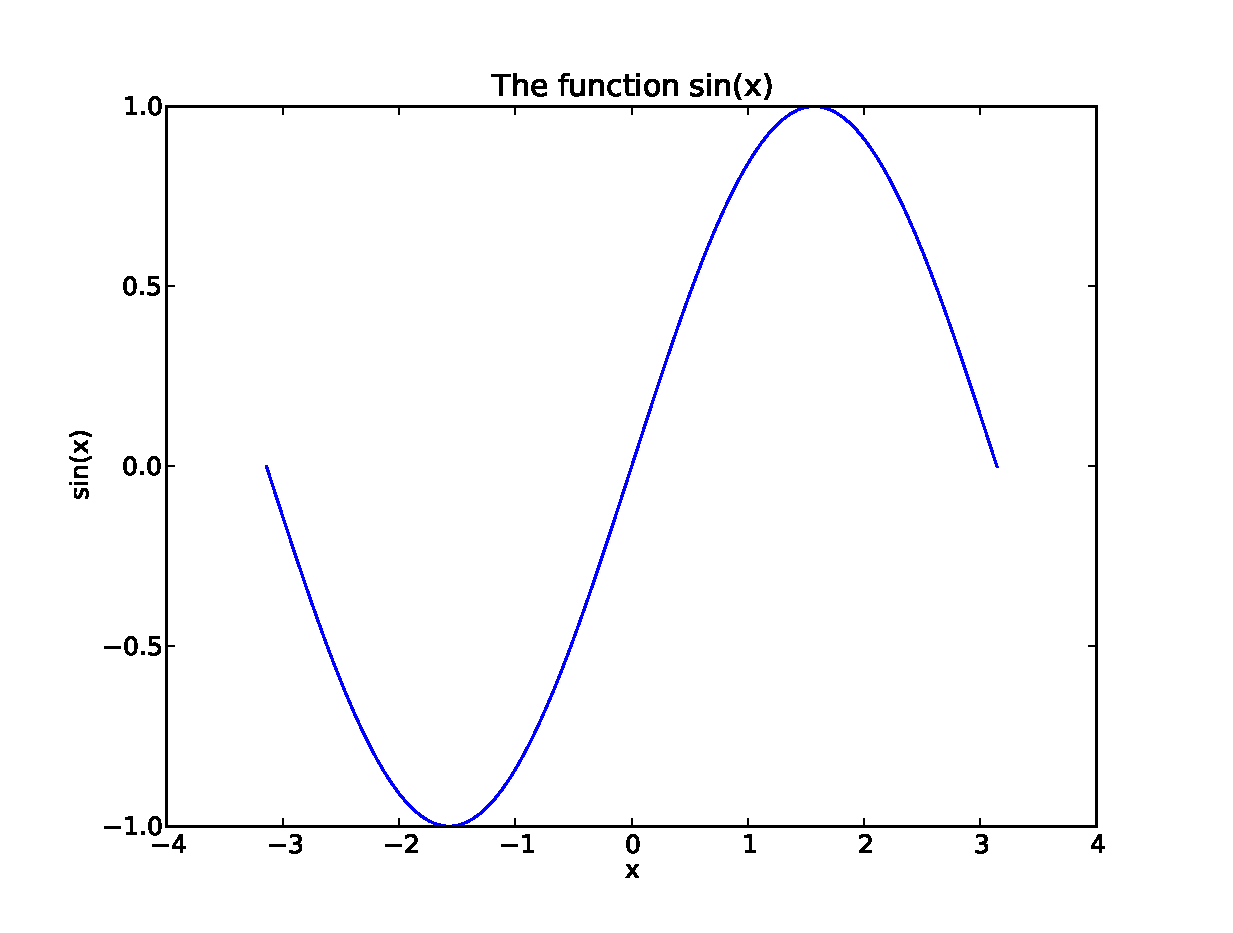
\epsfig{file=sine.eps, scale=0.6}} 
  \caption{A plot of the sine function in the interval $[-\pi, \pi]$.}
  \label{fig:sine.eps}
\end{figure}
There are lots of options to tweak the resulting figures.  Unfortunately, we do not have the time to
cover this topic in more depth.  Instead, I would encourage you to visit
\\[0.2cm]
\hspace*{1.3cm}
\href{http://matplotlib.org}{\texttt{http://matplotlib.org}}
\\[0.2cm]
for further information.
\end{document}



